% !TEX root = ../thesis.tex

\chapter{Background}
\label{ch:background}

In this chapter we describe existing technology that will be referred to throughout the paper.

\section{GitHub}

In this section we explore the pull request and issue features of GitHub.

\subsection{Issues}

GitHub issues is a useful feature for tracking, discussing and logging various issues/problems on a GitHub repository.
Any collaborator to a repository may open a GitHub issue, and describe any problem, idea or issue they have.
Other users may then contribute to the issue by commenting on it, easing the communication process within a project.
GitHub issues can therefore function as a discussion hub, and makes it especially useful for larger projects involving several people. 

\begin{figure}[ht]
    \centering
    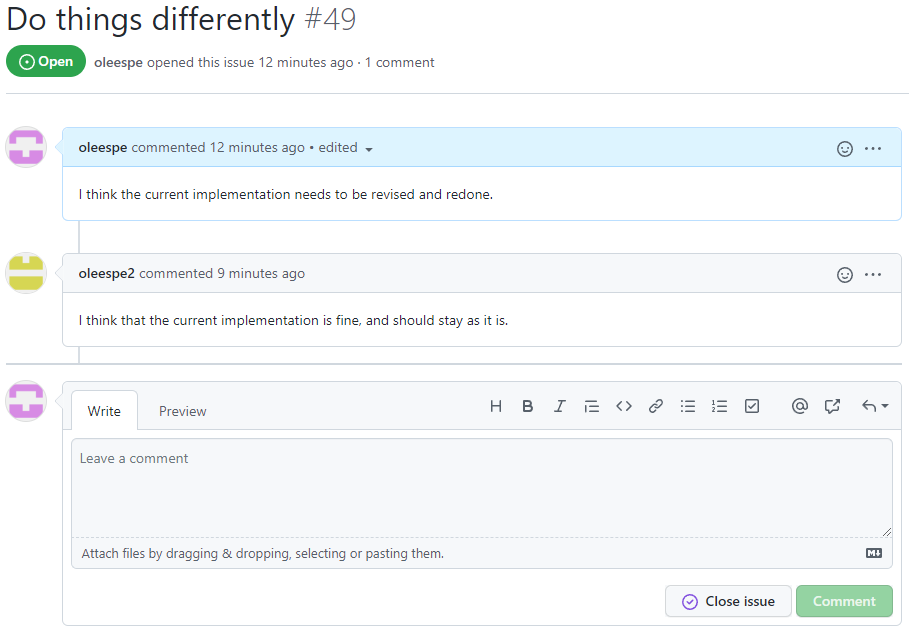
\includegraphics[width=\textwidth]{photos/github-issue.PNG}
    \caption{Example of a GitHub issue comment section}
    \label{fig:github-issue}
\end{figure}

\subsection{Pull requests}

Pull requests are a desire to merge any feature branch, into the main branch of a repository.
GitHub supports managing pull requests through its user interface, and allows any contributor to a repository to create a pull request.
Through the user interface, progress on a branch can be tracked, reviewed and commented on.
In this sense, GitHub pull requests function as a central hub for feature branches.

Code review is also a central part of GitHub pull requests.
Any eligible user may review, comment on and request changes to the source code of a given pull request.
The reviewer may also use reviews to approve a pull request for merging.

Pull requests can also be linked to issues.
Doing this will automatically associate any linked issue to the pull request, and cause them to close when the pull request closes.
A common workflow would be to create an issue, describing a problem, and then creating an associated pull request for this issue.

Through its features, GitHub pull requests provide an efficient way of implementing new features to any project.
As well as easing the communication of desired changes to any source code.

\begin{figure}[ht]
    \centering
    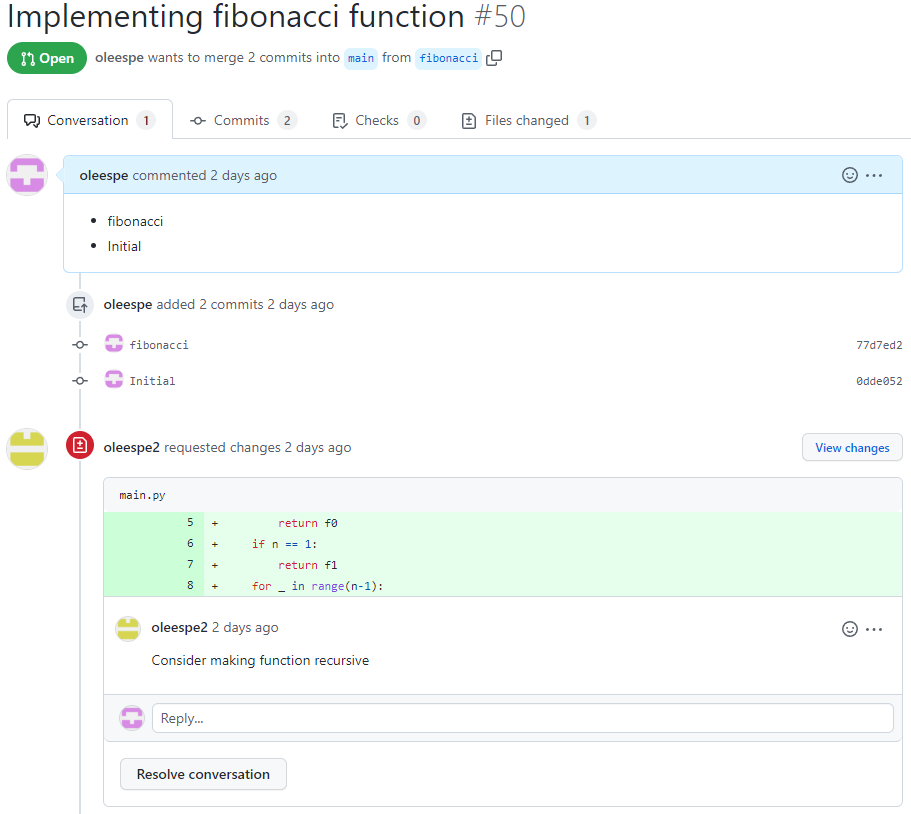
\includegraphics[width=\textwidth]{photos/pull-request.PNG}
    \caption{Example of parts of a GitHub pull request}
    \label{fig:pull-request}
\end{figure}

\subsection{Workflows}

Maybe maybe

\section{QuickFeed}

In this section we describe the features of QuickFeed that are important to this project.

\subsection{Protobuf}

Maybe maybe

\subsection{gRPC}

Maybe maybe

\subsection{Running tests on student code}

Maybe maybe

\subsection{QuickFeed repository structure}

When a teacher creates a course in QuickFeed, a GitHub organization is created to represent it.
Within this organization, three initial repositories are created, as well as student repositories when students enroll.
They are all described as follows:

\textit{info}: This repository simply holds information about a course.
The repository is available for all students, and would typically work as a simple information hub.

\textit{assignments}: The repository responsible for representing the assignments themselves.
Every assignment in a course is represented as a folder within this repository.
Students pull assignments from here, to their own local git repositories.

\textit{tests}: Within this repository every assignment is represented as a distinct folder.
The repository differs from \textit{assignments}, because contains specific assignment information, as well as test data.

Assignment information comes in the form of a \textit{assignment.yml} file, and should be present in every assignment folder.
Content within this file is used to generate the assignment itself, and may contain settings such as the assignment deadline.

Test data comes in the form of test code that should be run on the submitted student code.
Additionally, \textit{tests} may contain \textit{run.sh} script files, usually in a separate \textit{scripts} folder, or within each assignment folder.
The \textit{scripts} folder can also contain a Dockerfile, used to create a test environment.
The test code, script files and Dockerfile each contribute to how tests are run on student code.
Even though QuickFeed supports running automatic tests on student code, it is not required.
Assignments can simply contain no tests, leaving the assignments to have to be manually graded.
It is also worth noting that students never have access to this repository.


\begin{figure}[ht]
    \centering
    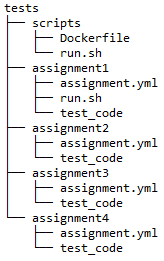
\includegraphics[scale=0.8]{photos/tests-repository-structure.PNG}
    \caption{Example of a tests repository folder structure}
    \label{fig:tests-repository-structure}
\end{figure}

Student repositories: There are two types of student repositories, user and group repositories.
Where a user, in this case, would simply be any student who has enrolled in the course, and a group is a multitude of students.
Their repository names follow the same format: \textit{name}-labs.
For an enrolled student, \textit{name} would be their GitHub user name.
A group's name however, would be defined by the group members themselves, when they enroll the group.

These repositories are the repositories students push their code to.
And it is this code that QuickFeed tests, scores and grades.


\begin{figure}[ht]
    \centering
    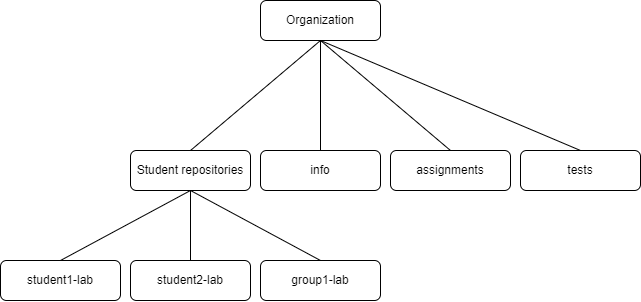
\includegraphics[width=\textwidth]{photos/qf-repository-structure.png}
    \caption{GitHub repository structure for a QuickFeed course}
    \label{fig:qf-repository-structure}
\end{figure}

\subsection{Webhooks}

QuickFeed communicates with GitHub in two ways.
In this section we will detail one of them, namely webhooks.

A webhook is a "user-defined callback over HTTP". % (ref: (09.04) https://developer.atlassian.com/server/jira/platform/webhooks/)
In general, webhooks allow developers to listen to events from any supporting sites.
When any such event occurs, an HTTP request is sent to the address configured for the webhook.
The request contains data about the event, usually in a JSON format.

QuickFeed uses webhooks to retrieve data from push events on a course.
When a new course is created, QuickFeed creates a webhook on the GitHub organization of the given course.
This webhook is only triggered by push events, which are then handled by QuickFeed accordingly:

\begin{itemize}
    \item If the push event is to the tests repository, QuickFeed will update the course assignments.
    \item If the push event is to a student repository, QuickFeed will determine the assignments that have been changed/worked on, 
    and run the assignment tests on them.
\end{itemize}

\subsection{SCM API}

The second way QuickFeed communicates with GitHub is through a custom API.

To facilitate communication with potentially any source control management system, a custom SCM API has been developed for QuickFeed.
The current iteration of QuickFeed supports interacting with GitHub through this API, via the go-github library. % (ref: go-github)
The library itself, communicates with GitHub's own REST API using HTTP requests.

The SCM API allows QuickFeed to perform various tasks, such as creating/updating repositories, creating webhooks, managing teams and more.
It, together with webhooks, therefore form a 2-way communication stream between QuickFeed and GitHub.